\documentclass{article}
\usepackage{graphicx} % Required for inserting images

\title{Estimating the Temperature of a Hohlraum}
\author{Isha Ankad, Paweł M. Kozłowski }
\date{July 2026}

\begin{document}

\maketitle




\section{Introduction}
In 2023, major milestones were met at the Lawrence Livermore National Laboratory (LLNL) Fusion facility with the occurrence of its first inertial confinement fusion. With this event, there's been a lot of excitement in the plasma physics community. This was done possible from the concentration of high-powered lasers in heating a hohlraum, which absorbed and emitted energy from the light as x-rays, within itself, repeatedly, creating an oven-like environment. It is crucial for experimentalists to know the quantities of such properties in order to foster environments that are sufficient to produce plasmic phenomenons to occur.  This project is aimed at estimating the temperatures of this hohlraum. Temperature of the hohlraum can be derived from the radiation. In this setup, there is another apparatus to account for in estimating the blackbody's temperature. A backlighter, a blackbody plate set at a distance from the hohlraum, where a subset of lasers power and cause the plate to emit x-rays directed towards the hohlraum and into a x-ray spectrometer. A dante diagnostic, in this system, is an appartus which is lowered over the hohlraum, and is used in recording the radiation signal from both the backlighter and the hohlraum. Readings from this diagnostic will be used in estimating the temperature of the hohlraum. In order to derive the temperature of the hohlraum, a model must be built which is able to disambiguate dante signal readings from the hohlraum and the backlighter. This is separated radiation from the hohlraum is able to produce an estimated temperature. Estimations of the signals will be created using Monte Carlo algorithms.
\begin{figure}
    \centering
    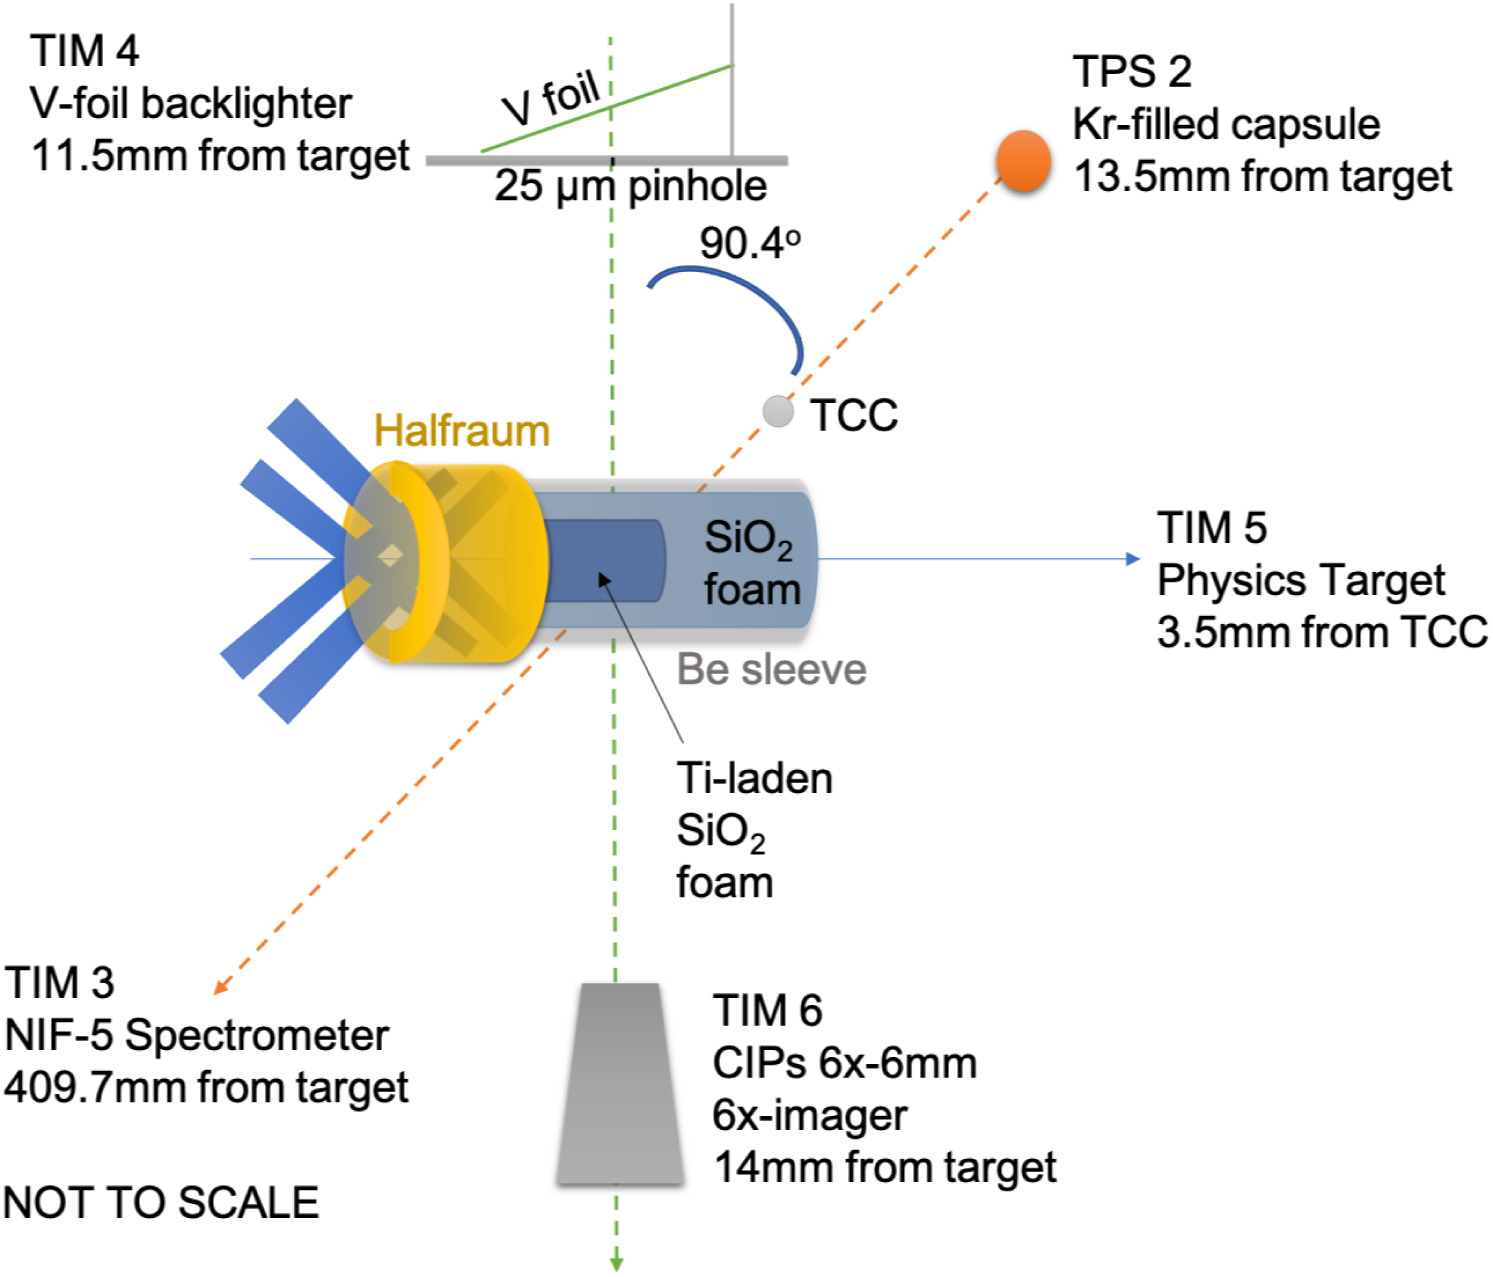
\includegraphics[width=0.5\linewidth]{images/apparatus.jpg}
    \caption{Symmetry and positioning of the different apparatus in a COAX platform}
    \label{fig:apparatus}
\end{figure}

\section{Background}
Radiation is emitted from multiple sources. The lasers that are aimed at the hohlraum (blackbody) cause it to absorb a high degree of energy which it outputs as x-rays. This energy is reabsorbed and re-emitted numerous times within the blackbody which is recorded as blackbody radiation by the dante diagnostic. Simultaneously, with the absorption of energy, the backlighter that is also powered by lasers, absorbs energy and re-emits this as x-ray, acting as a radiation source in the system. As a result of the exhibition of Blackbody and Bremsstrahlung radiation from the system, a mixed signal is picked from the dante diagnostic. Although, both radiations have unique behaviors with respect to photon energy that can be strategically used in differentiating the mixed signal.

\begin{figure}
    \centering
    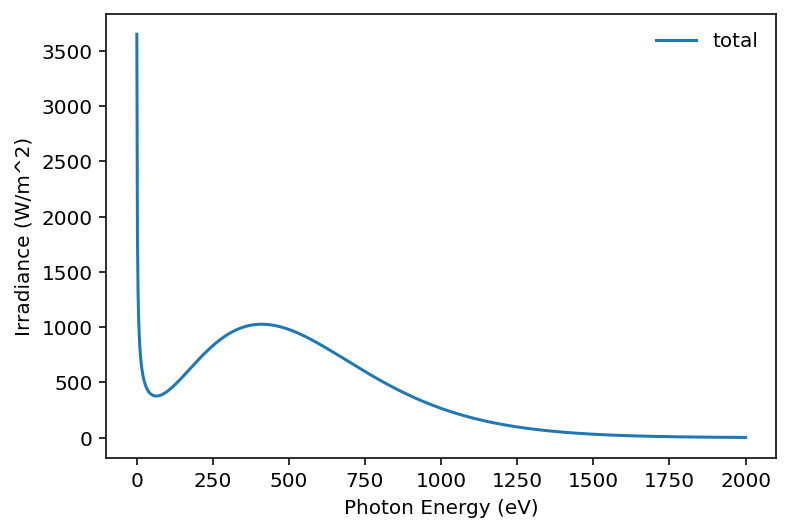
\includegraphics[width=0.5\linewidth]{images/updatedcurve.png}
    \footnotesize
    \caption{Figure 2 illustrates how an ideal reading of the Dante diagnostic would appear. Created using synthetically generated data.}
    \label{fig:dante_reading}
\end{figure}


\section{Methodology}

Variations of the Monte Carlo algorithm, such as the Metropolis Markov Chain (MCMC) and the Hamiltonian No U-turn Sampler (NUTS) will be used in the means of estimating blackbody properties. The model takes in prior knowledge (Prior) of how the different radiations uniquely behave with respective to photon energies and uses it to produce proposals that can be compared to the behavior of the measured data. The prior is a guess of what is desired of the model to estimate and this guess aids the model in its process of generating a proposal. 
After taking a prior, the model uses specific formulas to generate a proposed distribution of irradiance, for blackbody and bremsstrahlung separately, which it can use to compare directly with the measured data. 

In order to produce a proposal for the blackbody emission curve, the model would take in prior or guess temperature, and feed it into this formula, to generate an irradiance it will use to compare it to the measured data.

\vspace{5mm}
\begin{align}
    B_\nu(\nu, T) &= \frac{2h\nu^3}{c^2}\frac{1}{\exp\left(\frac{h\nu}{k_B T}\right) - 1} \\
    I_\nu(\nu, T) &= B_\nu(\nu, T)\,\frac{V}{D^2}
\end{align}
\vspace{5mm}

Similarly, by passing in this set of formulas into the model, it is able to generate an irradiance with an input of temperature. Here the bremsstrahlung coefficient is calculated in order to calculate how much power from the backlighter is recieved by a set surface area. 
\vspace{5mm}

\begin{align}
    j(\nu, T) &= \frac{8}{3}\sqrt{\frac{2\pi}{3 m_e k_B T}}\,\frac{e_c^6}{m_e c^3}\,Z^2 n_e n_i \, \exp\left(-\frac{E_p}{E_t}\right) \, \bar{g}_{ff} \\[6pt]
    \bar{g}_{ff} &= 1 + 0.1728\left(\frac{E_p}{I_H Z^2}\right)^{1/3}\left(1 + \frac{2E_t}{E_p}\right) \\[6pt]
    I &= \frac{j(\nu,T)\,V}{D^2}  
\end{align}

\vspace{5mm}

Using Bayes' Theorem in the equation above, Metropolis compares the variance between the distribution of the proposal and the measured, in order to determine whether to accept  or reject the proposal. 

\vspace{5mm}

\begin{block}{Bayes' Theorem}
    \centering
    P(A \mid B) = \frac{P(B \mid A) \, P(A)}{P(B)}
\end{block}
\vspace{5mm}


The further the proposed deviates from the measured the less likely it is to be accepted. The model uses the result and distribution of the previous proposal to shifts in values to arrive at a value which is less deviant from the measured and is of better likelihood. This proposal is then met with acceptance or rejection and the model is met with thousands of such draws which eventually arrive at the highest likely value of the measured. These accepted draws (samples) can be better illustrated as a distribution (posterior) where the low density areas/tails of the curve represent values quite deviant from the measured, thus less accepted and of low density.
\begin{figure}
    \centering
    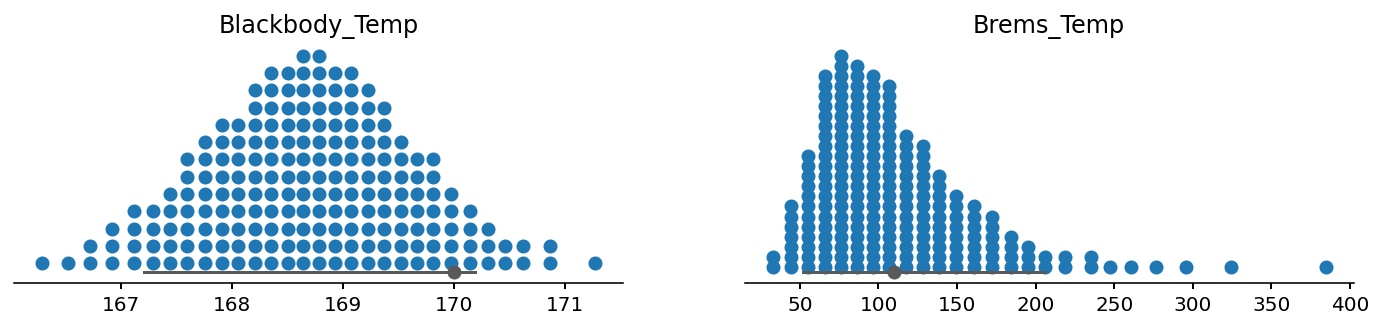
\includegraphics[width=0.5\linewidth]{images/posterior-new.png}
    \caption{Distribution of accepted draws or estimate values of the signals' temperatures}
    \label{fig:posterior}
\end{figure}

While, the most dense sections of the distribution, towards the mean, are the collection of samples closest to the measured values, making them more likely to be accepted and, as a result, they are more in abundance. The mean of the posterior distribution is the estimation of the measured value. The model guesses between different values of temperature, and compares that irradiance at a chosen temperature or proposal with the measured data, which allows the sample situated at the posterior’s mean to be easily tracked backed towards a temperature, allowing the model to achieve its purpose. This algorithm proves to be more efficient than a basic Accept-Reject Sampler because it uses its previous draw to propose a more favorable sample, pushing the sampler closer to the true value. The NUTS model uses a more direct and certain method in fitting measured values. It starts off similar to the Metropolis model, where a sample temperature guess is used in the calculation of irradiance, a value used to compare to the measured data. The model traces at what density the proposed guess lies on the distribution of the measured data. Then with the use of calculus, the model chooses to sample from the direction which has a greater slope, tangent to the curve, and continues sampling in such favor, eventually leading to the highest probable value, the true measured value.

\section{Choosing a model}
Amongst both models, the NUTS model performed significantly well compared to the Metropolis model. While both models could yield the accurate true measured temperature without difficulty, when introduced to noise, unavoidable in experimental data, the Metropolis model failed. With the implementation of an SNR system, where noise was varied to track model performance, NUTS model succeeded in fitting the measured values with the appropriate level of error respect to noise. This can be best illustrated with the tracking of the Mean Squared Error (MSE) over decreasing noise. The distance between the measured and fit is low correspond to high SNR values, where noise is low, thereby a good fit is expected. Conversely, the Metropolis Algorithm failed to show a meaningful trend of MSE values with respect to SNR values. In addition, the r-hat values that define how well chains convergence was around the value of 1 for the NUTS model, signifying well convergence, but ranged around 3-4 for the Metropolis mode, signifying weak convergence. Due to the difference in capabilities between the two models, it was appropriate to introduce the experimental values solely to the NUTS model. 

\begin{figure}
    \centering
    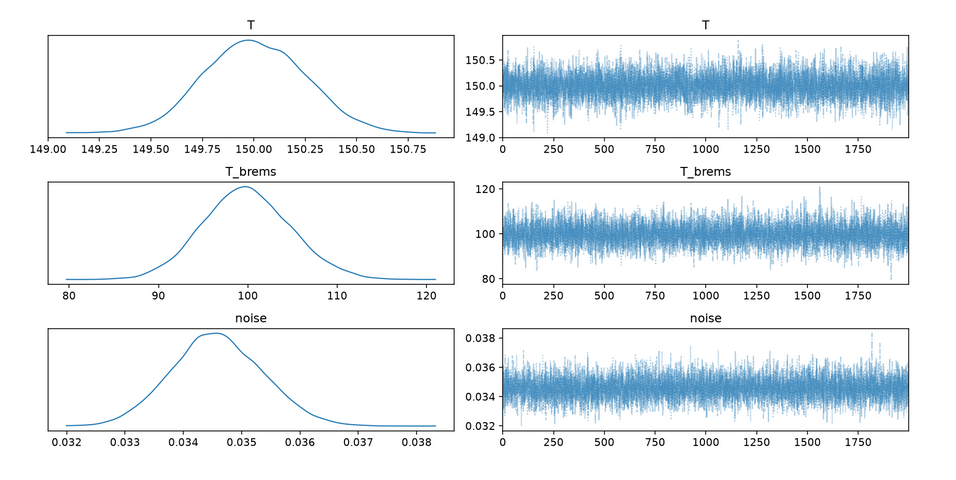
\includegraphics[width=0.5\linewidth]{images/hmc.png.png}
    \caption{Visualizing chain convergence and posterior distribution of the NUTS model}
    \label{fig:hmc}
\end{figure}


\begin{figure}
    \centering
    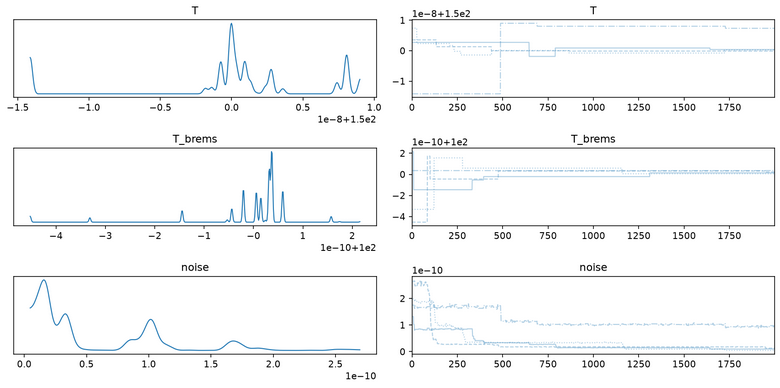
\includegraphics[width=0.5\linewidth]{images/metro.png}
    \caption{Visualizing chain convergence and posterior distribution of the Metropolis model}
    \label{fig:hmc}
\end{figure}


\section{Results}

Experimental data was used from the Dante diagnostic, which tracked change in power emission across different timesteps (nanoseconds). Unlike in the synthetic data generated to test the performance of the models, experimental Dante data has multiple peaks and rugged nature, with negative values which are labeled as unphysical. Simply using formulas to calculate irradiance for its comparison with this experimental data would not yield an accurate temperature. Instead, the model broke with the introduction of experimental data without any refinements. Thus, changes to the model became mandatory. It is worth to note that the fit created by the model will not fit the measured values due to its rugged nature and multiple peaks. The model will instead compromise the fit to create planckian curve defined by the formulas.

To understand the experimental data, Irradiance can be graphed against photon energies, producing a a set of emission curves.
\begin{figure}
    \centering
    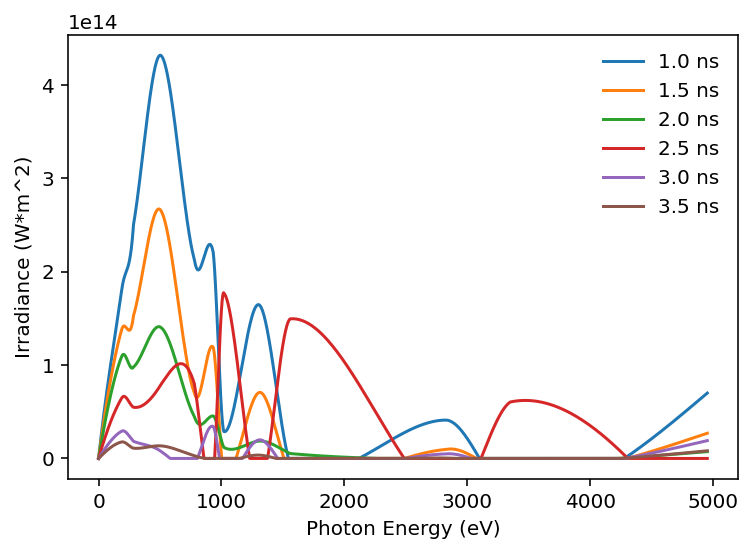
\includegraphics[width=0.5\linewidth]{images/fitdante.png}
    \label{fig:dante}
\end{figure}
In the figure above, it is of notice that the each curve, that represents the irradiance over photon energy at a set time step, precedes the emission curve of the prior nanosecond. This decreasing trend suggests that emission recorded is cooling over time. The cooling in energy is especially highlighted when comparing the posterior temperatures of the different temperatures over time steps. Although, the pattern over the time steps isn’t entirely uniform. There is a sudden spike in irradiance at the 2.5 nanosecond time step curve, notably around 2000 eV, not visible at any other step. The cause of this spike occurs due to the backlighter’s self-implosion with failure to sustain energy from the lasers. This implosion is recorded as a sudden spike in the system’s overall irradiation. This noise adds uncertainty in the model’s estimation of the blackbody’s internal properties.







\section{Handling Errors}

With the addition of the experimental data, the NUTS toy model proves unsuitable because it consists of strict parameters that restrain the variables relevant to the calculation of irradiance. Thereby, if experimental data had unexpected dips in irradiance at certain photon energies, the preset formulas that calculate irradiance are simply going to propose a smooth planckian curve, causing the model to neglect all of its proposals since they cannot fit the rugged measured data. The solution in making the model more flexible is to add an amplitude term, that provides the model a cushioning, allowing it to even accept proposals that notably deviate from the experimental data. The number of divergences that were abundant prior to the addition of the amplitude term drops to 0. Divergences refer to areas of high curvature where the model fails to grasp the next step or draw. With the addition of an amplitude term, the areas with high curvatures are diluted, preventing divergences to occur. Additionally, given the presence of unphysical values, the experimental data had to be half normalizing between the range of 0 and 1, otherwise, unfiltered data would cause the model to break.   



                  
\section{Future Work}

Further measures may be taken to improve the readings of the model. The figure below shows the model's estimates of the shapes of the signal curves. Given that the total and the blackbody emission curves overlap entirely, the model almost neglects fitting the bremsstrahlung radiation. This failure of the model can be a point for further development in order for it to also account for bremsstahlung radiation. Additionally, instead of creating an additional parameter to act as an amplitude term, existing variables that play a role in defining the magnitude of irradiance could be normally distributed with respect to their usual value. Another change could be to account for the disruption in irradiance caused by the backlighter’s implosion, and separating it from the total emission curve. This way the estimations of the internal properties for the different radiations are met with more accuracy and certainty. Additionally, this project only analyzes two models, thereby, other Bayesian models can provide further insight on better data reading and analysis. 

\begin{figure}
    \centering
    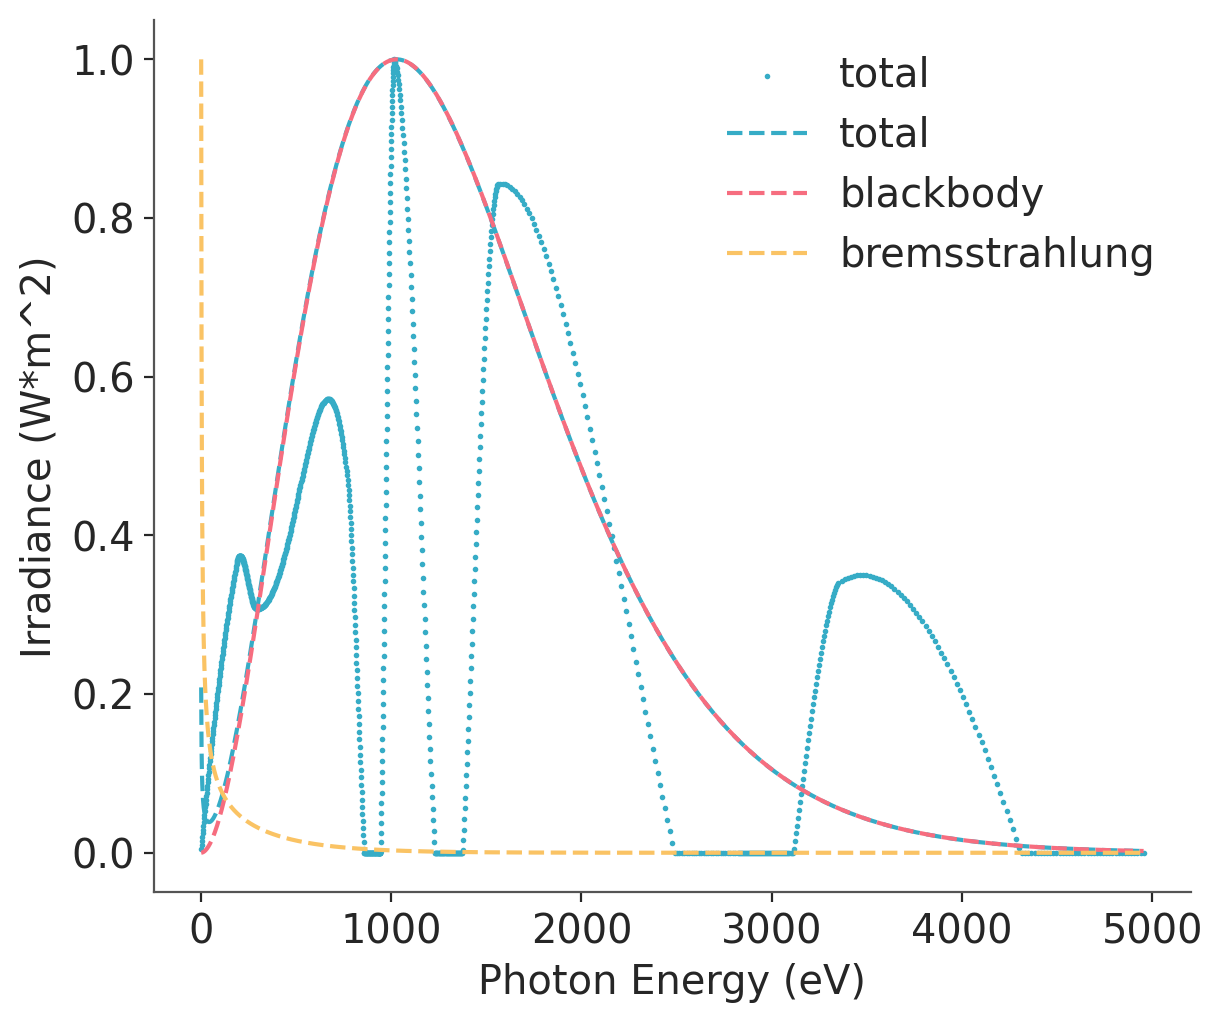
\includegraphics[width=0.5\linewidth]{images/fit_of_all_curves.png}
    \label{fig:placeholder}
\end{figure}
                                  
\section{Conclusion}

In conclusion, the objective in finding the internal properties of a blackbody can be estimated using mathematical algorithms that analyze measured data and propose distribution of the likelihood of values being equal to the measured value. After comparing the performance of two Bayesian models, it was found that the NUTS model using Hamiltonian Monte Carlo excelled in estimating synthetically made values, given its high chain convergence and good fit metric values. The model performed contextually well with varied levels of noise using synthetically generated values. Although this model wasn't able to succeed when estimating experimental data from real dante readings, due to its failure in accounting for bremsstrahlung's radiation. The addition of an amplitude term as well as the normalization of data was needed to illustrate the model better and allowing it to be more flexible in accepting draws. With these changes the model was less fragile and sensitive to the rugged nature of the Dante diagnostic readings, but as a result, the model compromised accounting for the irradiance values where experimental data deviated from a planckian shape, increasing uncertainty in its estimation. 




\section{Works Cited}
\footnotesize
\begin{itemize}
    \item National Ignition Facility & Photon Science (2026). Capsule Implosions | National Ignition Facility & Photon Science.
    \item Science Direct. “High Energy Density Physics.”
    \item National Ignition Facility & Photon Science. "Achieving Fusion Ignition."
    \item Samplers | PyMC v5.3.1 documentation. pymc.io
\end{itemize}

\end{document}
